% --------------------------------------------------------------------------- %
% Poster for the ECCS 2011 Conference about Elementary Dynamic Networks.      %
% --------------------------------------------------------------------------- %
% Created with Brian Amberg's LaTeX Poster Template. Please refer for the     %
% attached README.md file for the details how to compile with `pdflatex`.     %
% --------------------------------------------------------------------------- %
% $LastChangedDate:: 2011-09-11 10:57:12 +0200 (V, 11 szept. 2011)          $ %
% $LastChangedRevision:: 128                                                $ %
% $LastChangedBy:: rlegendi                                                 $ %
% $Id:: poster.tex 128 2011-09-11 08:57:12Z rlegendi                        $ %
% --------------------------------------------------------------------------- %
\documentclass[a0paper,portrait]{baposter}

\usepackage[ngerman]{babel}
\usepackage{relsize}		% For \smaller
\usepackage{url}			% For \url
\usepackage{epstopdf}	% Included EPS files automatically converted to PDF to include with pdflatex
\usepackage{tikz}
\usepackage{blindtext,multicol,fontspec}
%\setmainfont{Linux Libertine O}

%%% Global Settings %%%%%%%%%%%%%%%%%%%%%%%%%%%%%%%%%%%%%%%%%%%%%%%%%%%%%%%%%%%

\graphicspath{{Bilder/}}	% Root directory of the pictures 
\tracingstats=2			% Enabled LaTeX logging with conditionals

%%% Color Definitions %%%%%%%%%%%%%%%%%%%%%%%%%%%%%%%%%%%%%%%%%%%%%%%%%%%%%%%%%

\definecolor{bordercol}{RGB}{40,40,40}
\definecolor{headercol1}{RGB}{150,200,255}
\definecolor{headercol2}{RGB}{72,61,139}
\definecolor{headerfontcol}{RGB}{0,0,0}
\definecolor{boxcolor}{RGB}{240,270,255} %%gut: 230:291:255
\definecolor{boxColorTwo}{RGB}{80,80,80}
\definecolor{bgColor1}{RGB}{235,255,250}
\definecolor{bgColor2}{RGB}{70,70,255}

%%%%%%%%%%%%%%%%%%%%%%%%%%%%%%%%%%%%%%%%%%%%%%%%%%%%%%%%%%%%%%%%%%%%%%%%%%%%%%%%
%%% Utility functions %%%%%%%%%%%%%%%%%%%%%%%%%%%%%%%%%%%%%%%%%%%%%%%%%%%%%%%%%%

%%% Save space in lists. Use this after the opening of the list %%%%%%%%%%%%%%%%
\newcommand{\compresslist}{
	\setlength{\itemsep}{1pt}
	\setlength{\parskip}{0pt}
	\setlength{\parsep}{0pt}
}

%%%%%%%%%%%%%%%%%%%%%%%%%%%%%%%%%%%%%%%%%%%%%%%%%%%%%%%%%%%%%%%%%%%%%%%%%%%%%%%
%%% Document Start %%%%%%%%%%%%%%%%%%%%%%%%%%%%%%%%%%%%%%%%%%%%%%%%%%%%%%%%%%%%
%%%%%%%%%%%%%%%%%%%%%%%%%%%%%%%%%%%%%%%%%%%%%%%%%%%%%%%%%%%%%%%%%%%%%%%%%%%%%%%

\begin{document}
\typeout{Poster rendering started}

%%% Setting Background Image %%%%%%%%%%%%%%%%%%%%%%%%%%%%%%%%%%%%%%%%%%%%%%%%%%
%\background{
%	\begin{tikzpicture}[remember picture,overlay]%
%	\draw (current page.north west)+(-2em,2em) node[anchor=north west]
%	{\includegraphics[height=1.1\textheight]{background}};
%	\end{tikzpicture}
%}

%%% General Poster Settings %%%%%%%%%%%%%%%%%%%%%%%%%%%%%%%%%%%%%%%%%%%%%%%%%%%
%%%%%% Eye Catcher, Title, Authors and University Images %%%%%%%%%%%%%%%%%%%%%%
\begin{poster}{
	grid=false,
	% Option is left on true though the eyecatcher is not used. The reason is
	% that we have a bit nicer looking title and author formatting in the headercol
	% this way
	eyecatcher=true, 
	borderColor=bordercol,
	headerColorOne=headercol1,
	headerColorTwo=headercol2,
	headerFontColor=headerfontcol,
	% Only simple background color used, no shading, so boxColorTwo isn't necessary
	boxColorOne=boxcolor,
	boxColorTwo=headercol2,
	headershape=roundedright,
	headerfont=\Large\sf\textbf,
	textborder=rectangle,
	%background=user,
	headerborder=open,
	bgColorOne=bgColor1,
	bgColorTwo=bgColor2,
	background=shadeTB,
	%headershade=shadeTB,
  	%boxshade=shadeTB,
}
%%% Eye Cacther %%%%%%%%%%%%%%%%%%%%%%%%%%%%%%%%%%%%%%%%%%%%%%%%%%%%%%%%%%%%%%%
{
	%Eye Catcher, empty if option eyecatcher=false - unused
%\hspace{-3.5cm}
\setlength\fboxsep{0pt}
\setlength\fboxrule{0.5pt}
\fbox{
\begin{minipage}{10em}
	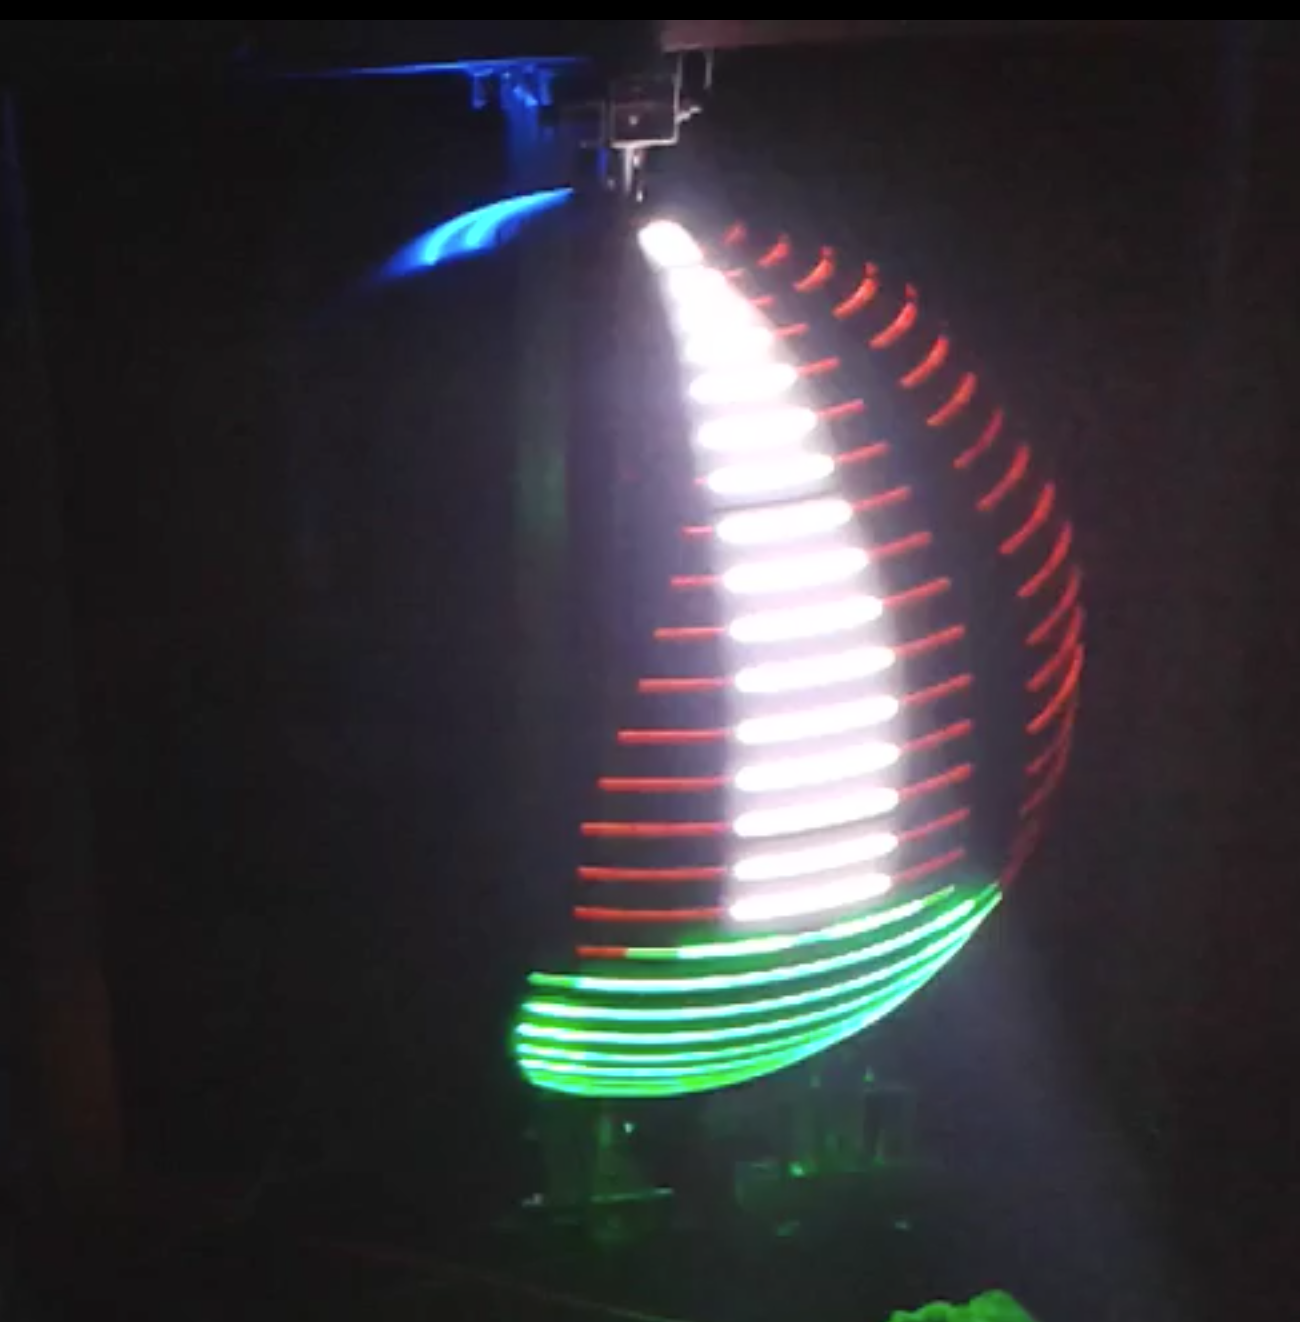
\includegraphics[width=10em]{globe}
\end{minipage}
}
}
%%% Title %%%%%%%%%%%%%%%%%%%%%%%%%%%%%%%%%%%%%%%%%%%%%%%%%%%%%%%%%%%%%%%%%%%%%
{
\sf\textbf{\hspace{-4.5em} POV-Globe}
}
%%% Authors %%%%%%%%%%%%%%%%%%%%%%%%%%%%%%%%%%%%%%%%%%%%%%%%%%%%%%%%%%%%%%%%%%%
{
	\hspace{-7.5em}
	\vspace{1em} Maximilian Hartmann, Philipp Gernandt, Tobias Buck\\
	\hspace{-7.5em}
	{\smaller Betreuer: Gero Plettenberg und Thomas Kloepfer}
}
%%% Logo %%%%%%%%%%%%%%%%%%%%%%%%%%%%%%%%%%%%%%%%%%%%%%%%%%%%%%%%%%%%%%%%%%%%%%
{
% The logos are compressed a bit into a simple box to make them smaller on the result
% (Wasn't able to find any bigger of them.)
\hspace{-3.5cm}
\setlength\fboxsep{0pt}
\setlength\fboxrule{0.5pt}
	\fbox{
		\begin{minipage}{10em}
			
\includegraphics[width=10em]{iwr.png}
%			\includegraphics[width=4em,height=4em]{elte_logo} \\
%			\includegraphics[width=10em,height=4em]{dynanets_logo}
%			\includegraphics[width=4em,height=4em]{aitia_logo}
		\end{minipage}
	}
}

\headerbox{Projektziel}{name=Ziel,column=0,row=0}{
Die Zielsetzung unseres Projektes bestand darin, aus einer runden, rotierenden RGB LED-Zeile einen Bildschirm zu konstruieren. Das besondere dabei ist, dass bei Rotation der LED-Zeile sich ein kugelförmiger Bildschirm ergibt. Wir benutzen ein Raspberry-Pi um PNG Bilder einzulesen und die Rotation der LED-Zeile zu steuern.\\
Dabei soll das Bild stabil angezeigt werden ohne davon zu wandern. Außerdem sollen Funktionen zum Einfachen einlesen und Anzeigen von Bildern erstellt werden.
%\includegraphics[width=\linewidth]{time_windows}
}

\headerbox{Umsetzung}{name=ums,column=0,below=Ziel}{
Unsere Idee wurde umgesetzt indem wir eine Aluminiumhalterung samt rotierendem LED-Kreis durch einen Standventilatormotor antreiben. Als LED-Zeile haben wir einen adressierbaren LED-Schlauch von Adafruit Industries (Adafruit DotStar) benutzt, was das Ansprechen der LEDs wesentlich vereinfacht. Dies ergibt 60 Pixel vom Nord- zum Südpol der Kugel. Die LED-Zeile und die Synchronisation der Anzeigefrequenz mit der Drehfrequenz des Motors wird durch ein Raspberry-Pi gesteuert. Unser Programm haben wir in Python geschrieben.
\begin{center}
	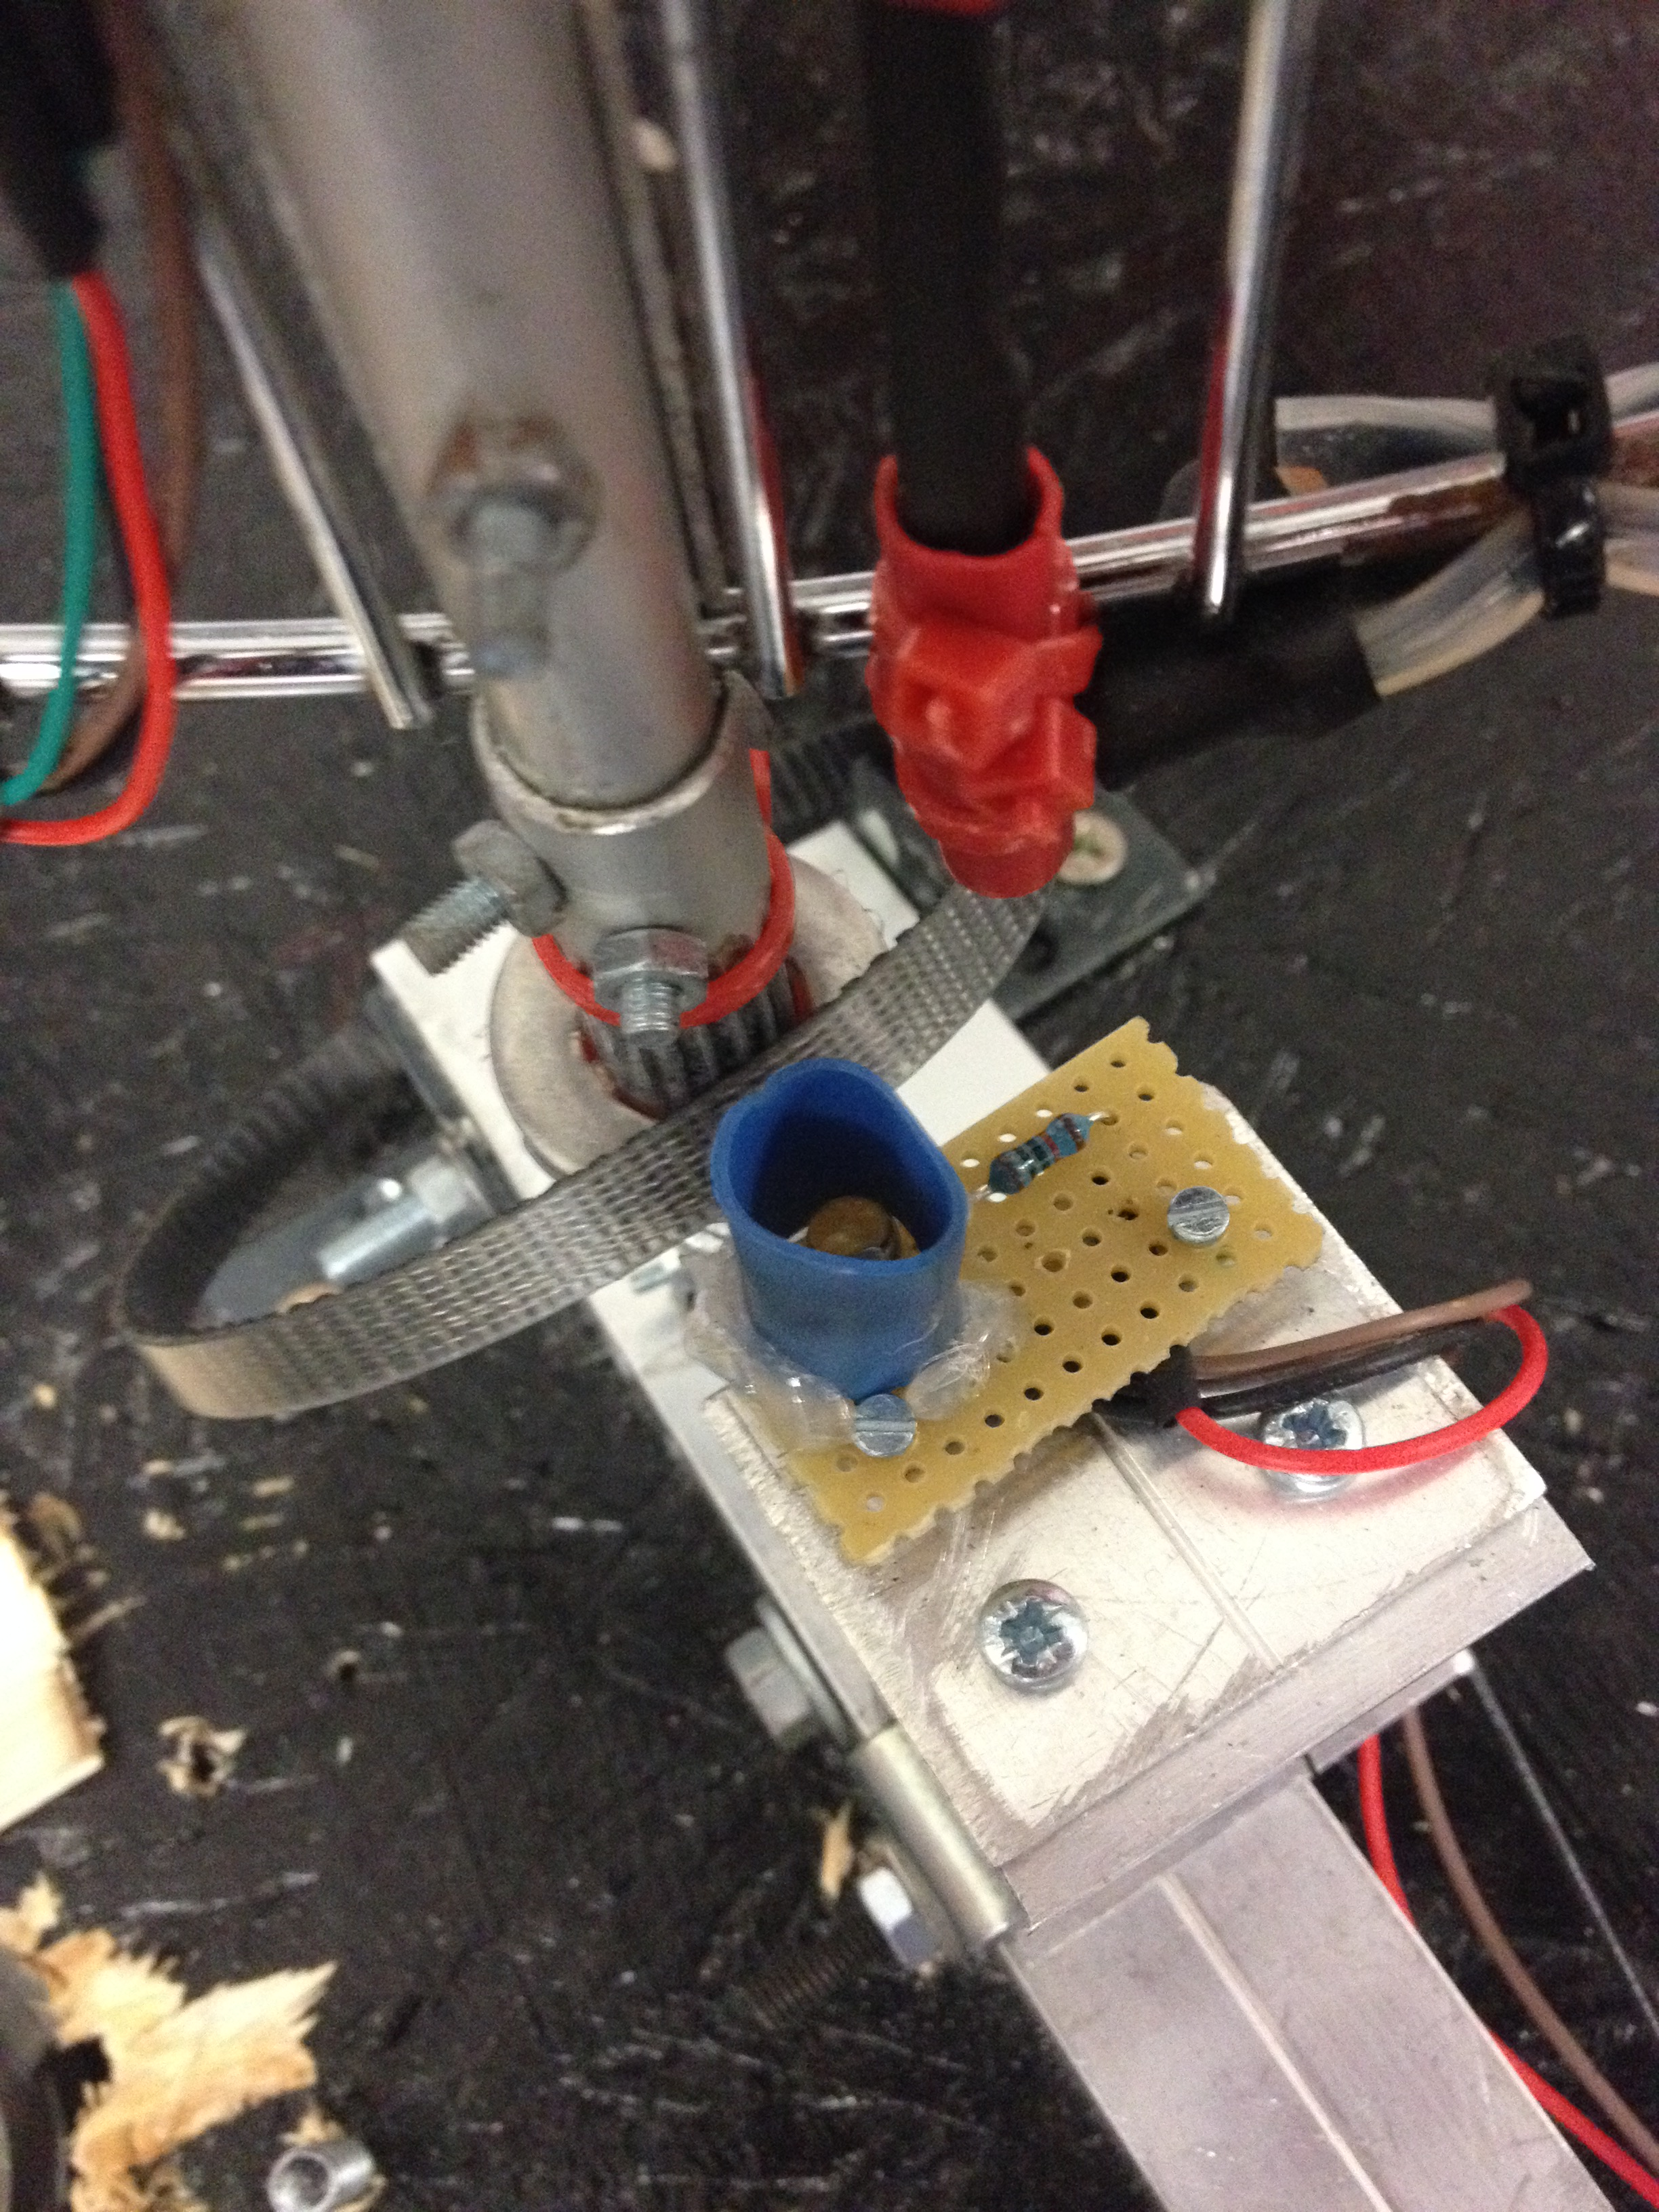
\includegraphics[width=\columnwidth]{Photodiode}
\end{center}
}

\headerbox{POV}{name=POV,column=0,below=ums,above=bottom}{
Das Prinzip von POV (Persistence of vision) beruht darauf, dass das Auge Reize nur mit einer bestimmten Frequenz verarbeiten kann, z.B. Filme nur mit 24Hz und Cartoons mit 12Hz. Alles was sich schneller als mit 24Hz ändert ist für das Auge nicht wahrnehmbar. Das bedeutet, eine schnell bewegte Lichtquelle erscheint beispielsweise als Linien und eine blinkende erscheint als mehrere Pixel. Somit erscheint unsere schnell bewegte gekrümmte LED-Zeile als eine mit farbigen Pixeln besetzte Kugeloberfläche. "Blinken nun alle LEDs zur richtigen Zeit", synchron mit der Drehfrequenz, dann erhält man einen kugelförmigen Bildschirm.
}

%\vspace{1cm}
%\smaller													% Make the whole text smaller
%\vspace{-0.4em} 										% Save some space at the beginning
%\bibliographystyle{plain}							% Use plain style
%\renewcommand{\section}[2]{\vskip 0.05em}		% Omit "References" title
%\begin{thebibliography}{1}							% Simple bibliography with widest label of 1
%\itemsep=-0.01em										% Save space between the separation
%\setlength{\baselineskip}{0.4em}					% Save space with longer lines
%\bibitem{flöte} Flötenroboter Semester \emph{Projektname}, Webseite
%\end{thebibliography}


\headerbox{Aufbau des Roboters}{name=Aufbau,span=2,column=1,row=0}{
\begin{multicols}{2}
Der POV-Roboter besteht aus einer runden LED-Zeile mit 60 LEDs, montiert an eine Drehachse, die durch eine Standventilatormotor betrieben wird. Gesteuert wird der Roboter durch eine Raspberry Pi und die Daten werden über einen 4-poligen (Vcc, Gnd, Data, Clock) Klinkenstecker auf die rotierenden Komponenten übertragen. Eine Photodiode misst die Drehfrequenz und lässt somit die Synchronisation zwischen Drehfrequenz der LED-Zeile und Anzeigefrequenz zu.
\begin{center}
\vspace{-.5cm}
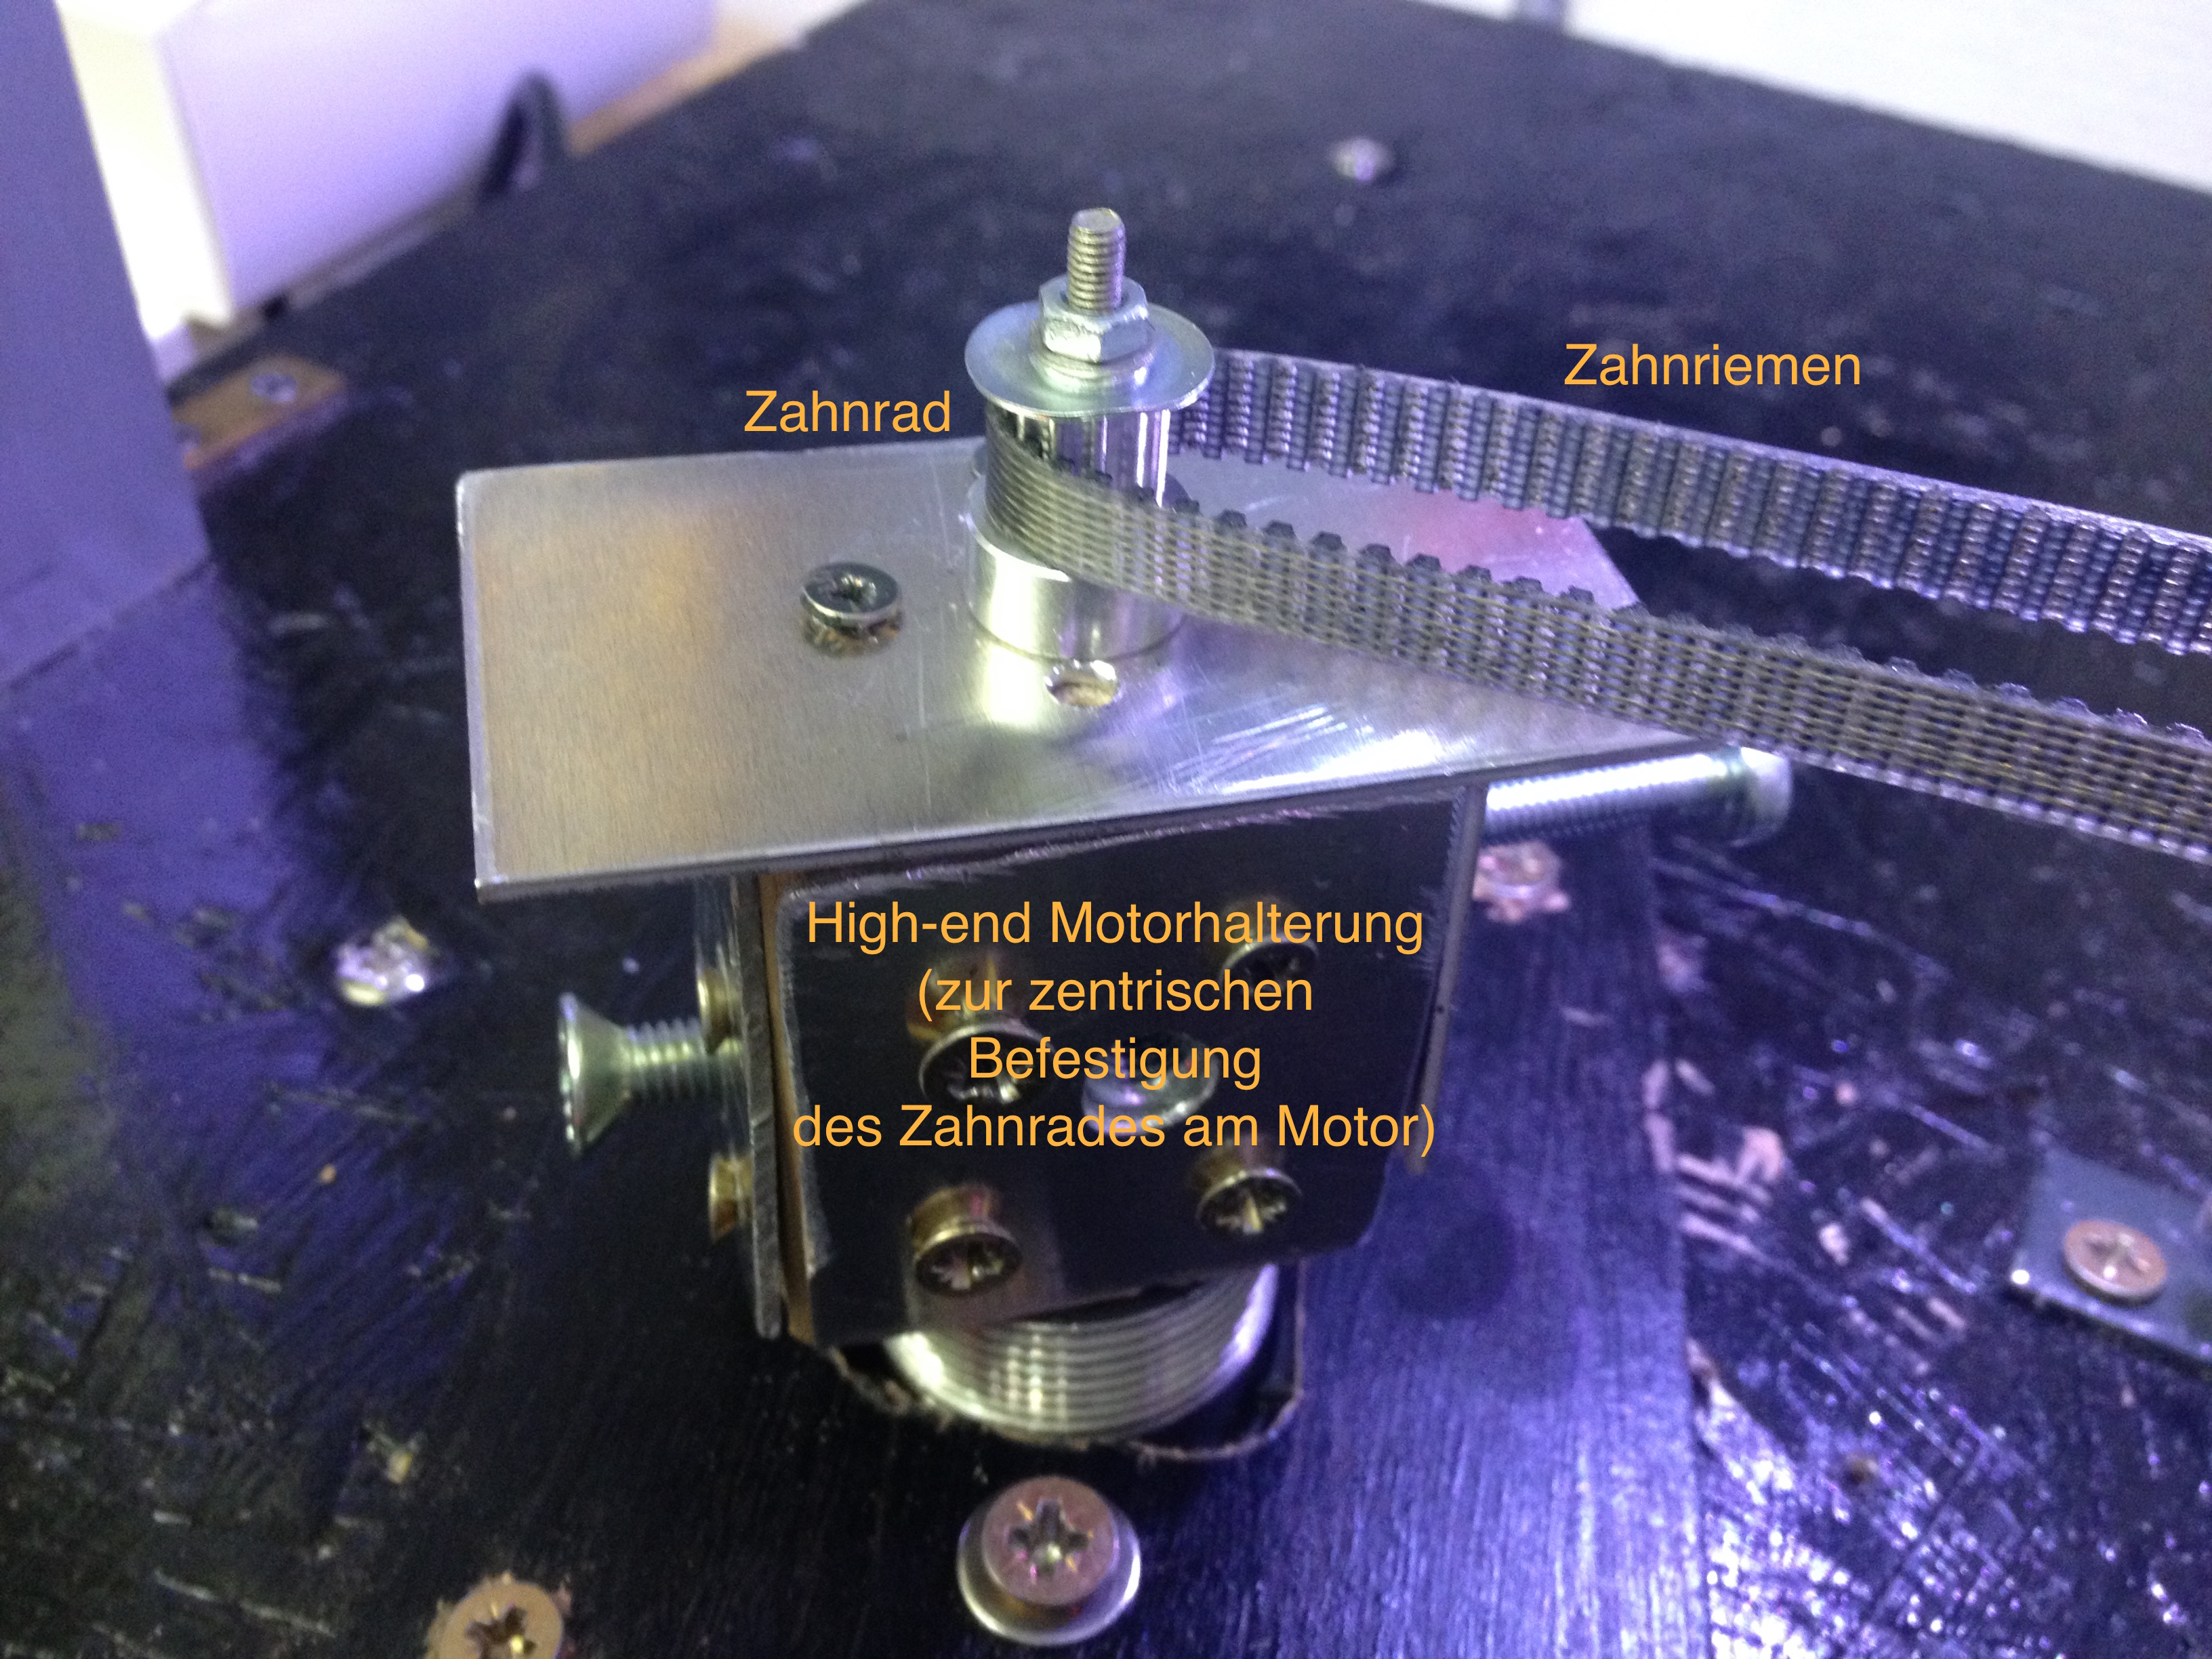
\includegraphics[width=7.5cm]{Motor_oben}
\end{center}
\columnbreak
\begin{center}
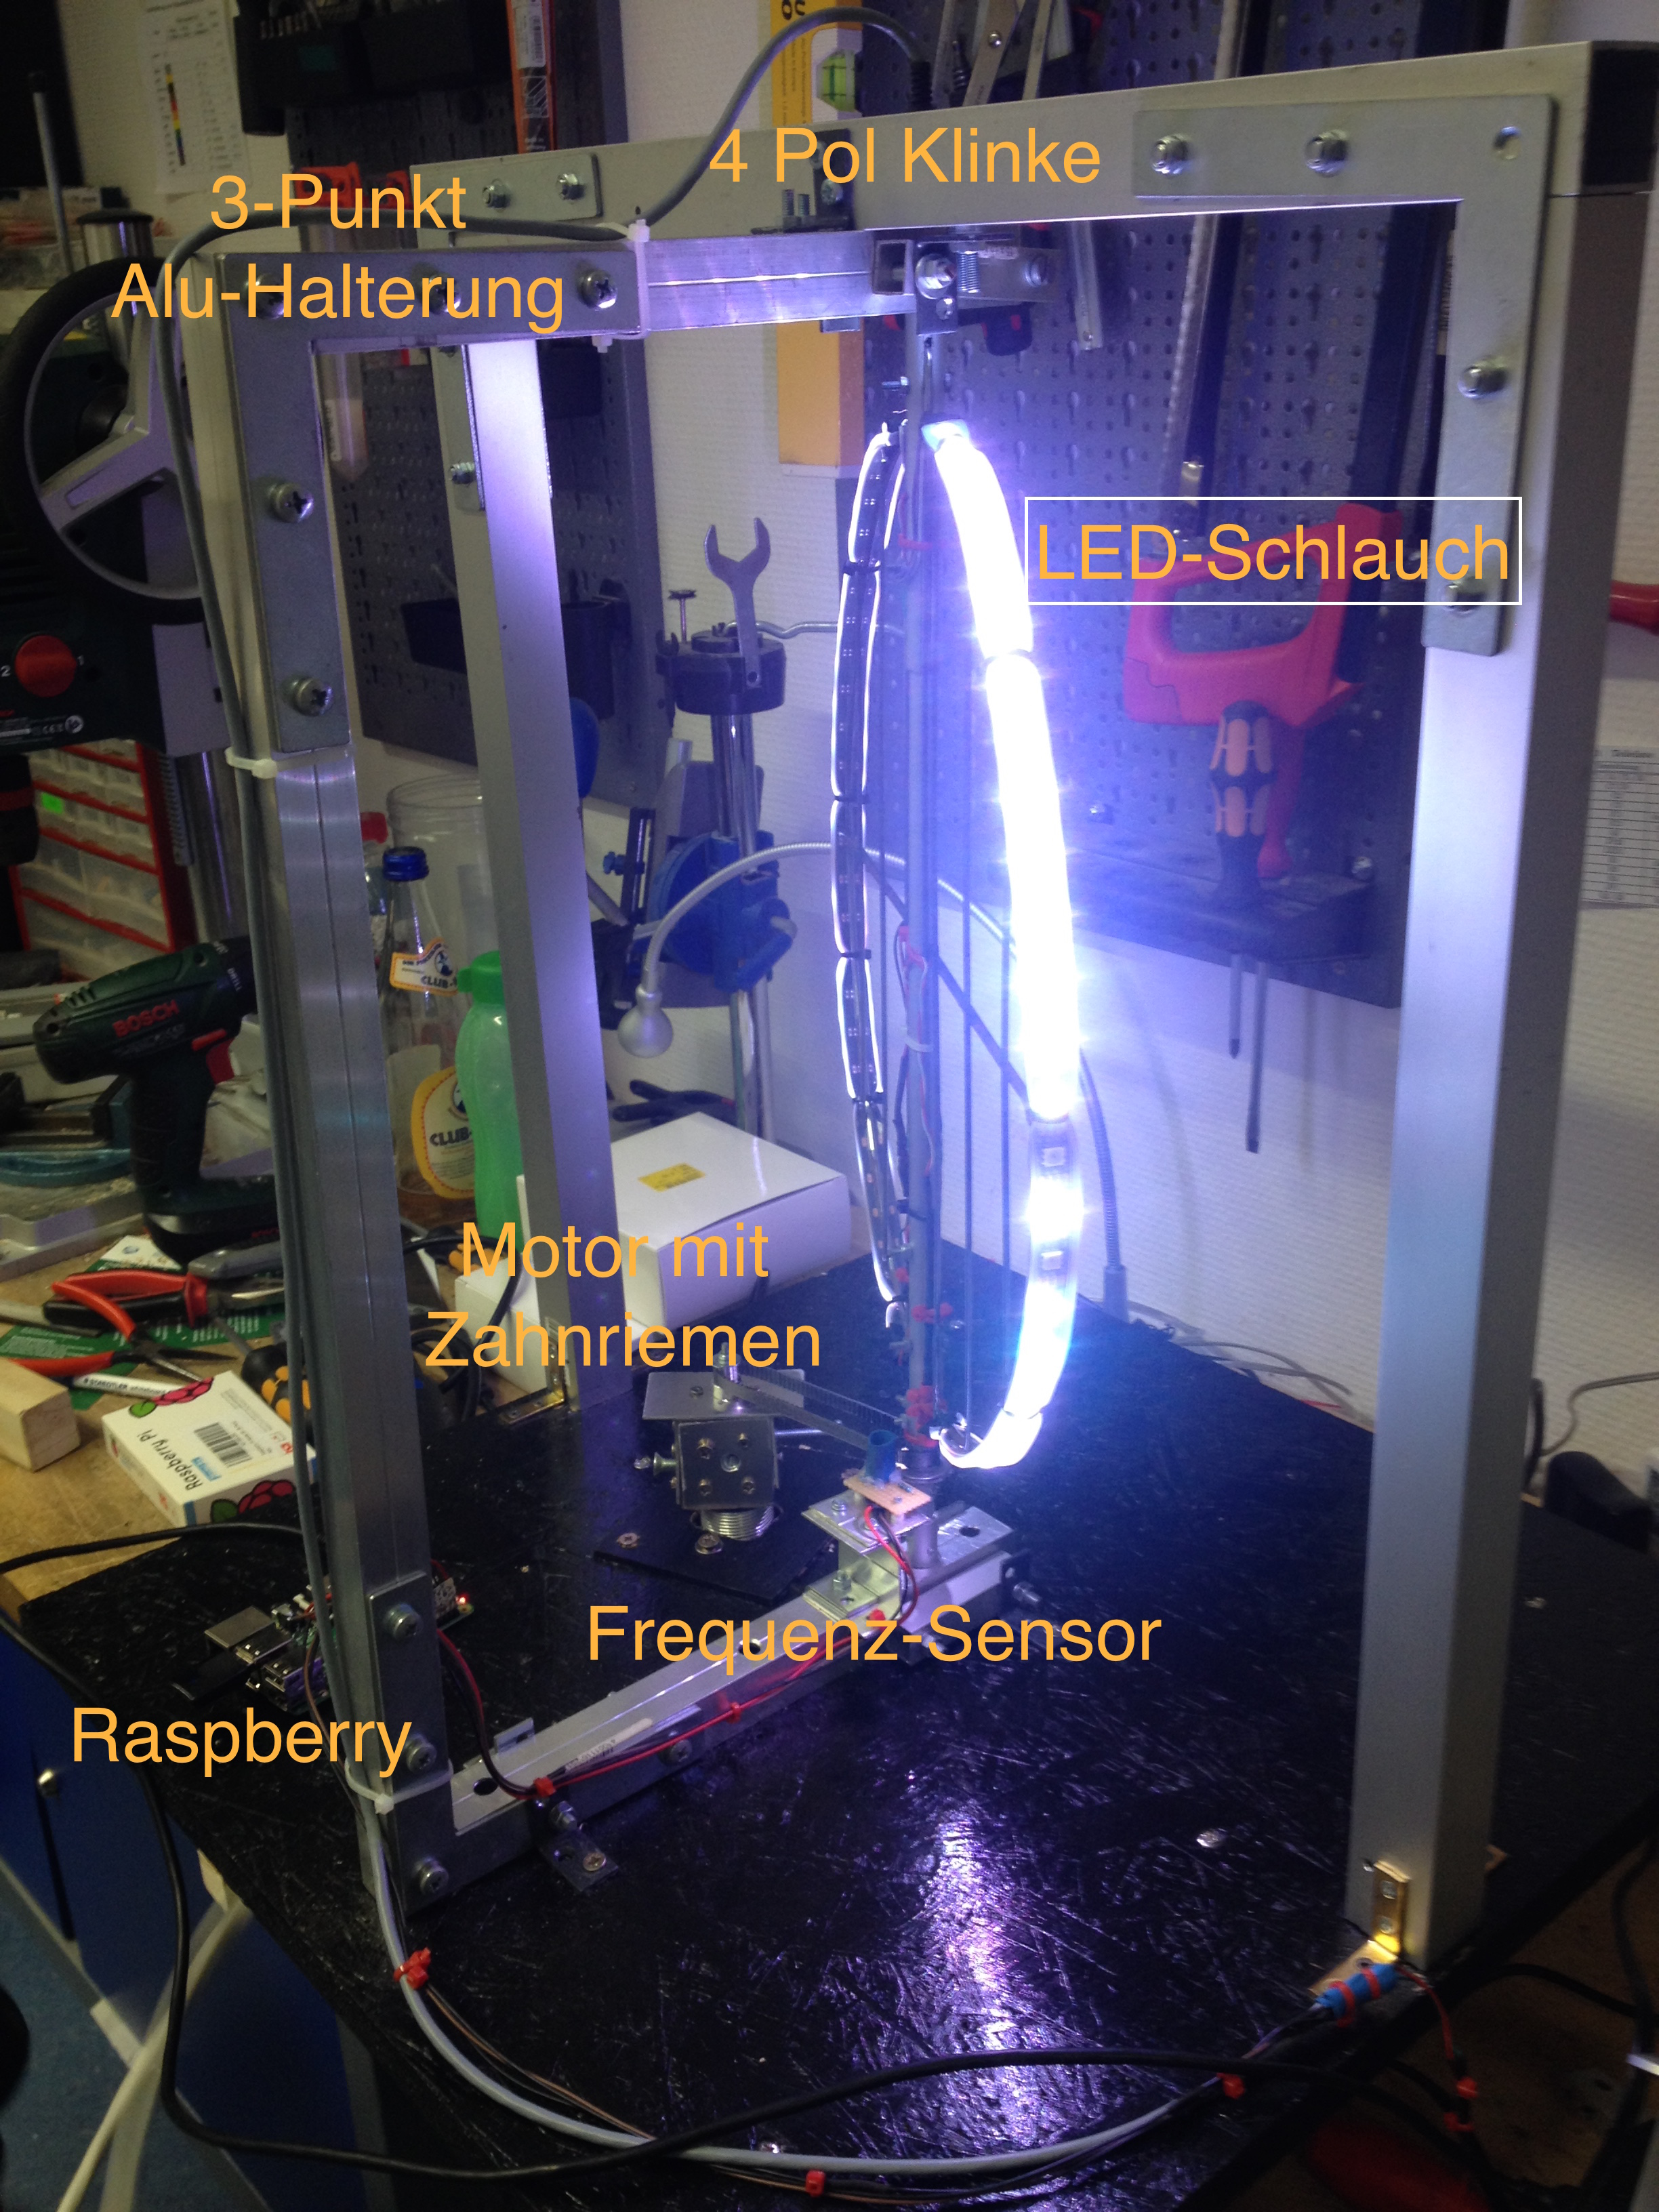
\includegraphics[width=7.5cm]{Komponenten}
%\includegraphics[trim=0cm 0.1cm 0.2cm 0.2cm, clip=true,width=0.65\linewidth]{Aufbau.pdf}
\end{center}
\end{multicols}
}

\headerbox{Steuerung}{name=konzept,span=2,column=1,below=Aufbau}{
Die Steuerung des Roboters und die Anzeige von Bildern wird durch einen Raspberry Pi übernommen. Das Programm kann PNG Bilder einlesen und die Zeilen und Spalten des Bildes an das Layout unseres Roboters anpassen. Somit kann zu jedem Zeitpunkt jeweils eine Spalte des Bildes durch die LED-Zeile angezeigt werden. Dabei wurde unter anderem auch die von Adafruit bereitgestellte Library für den LED-Schlauch benutzt.
\begin{center}
	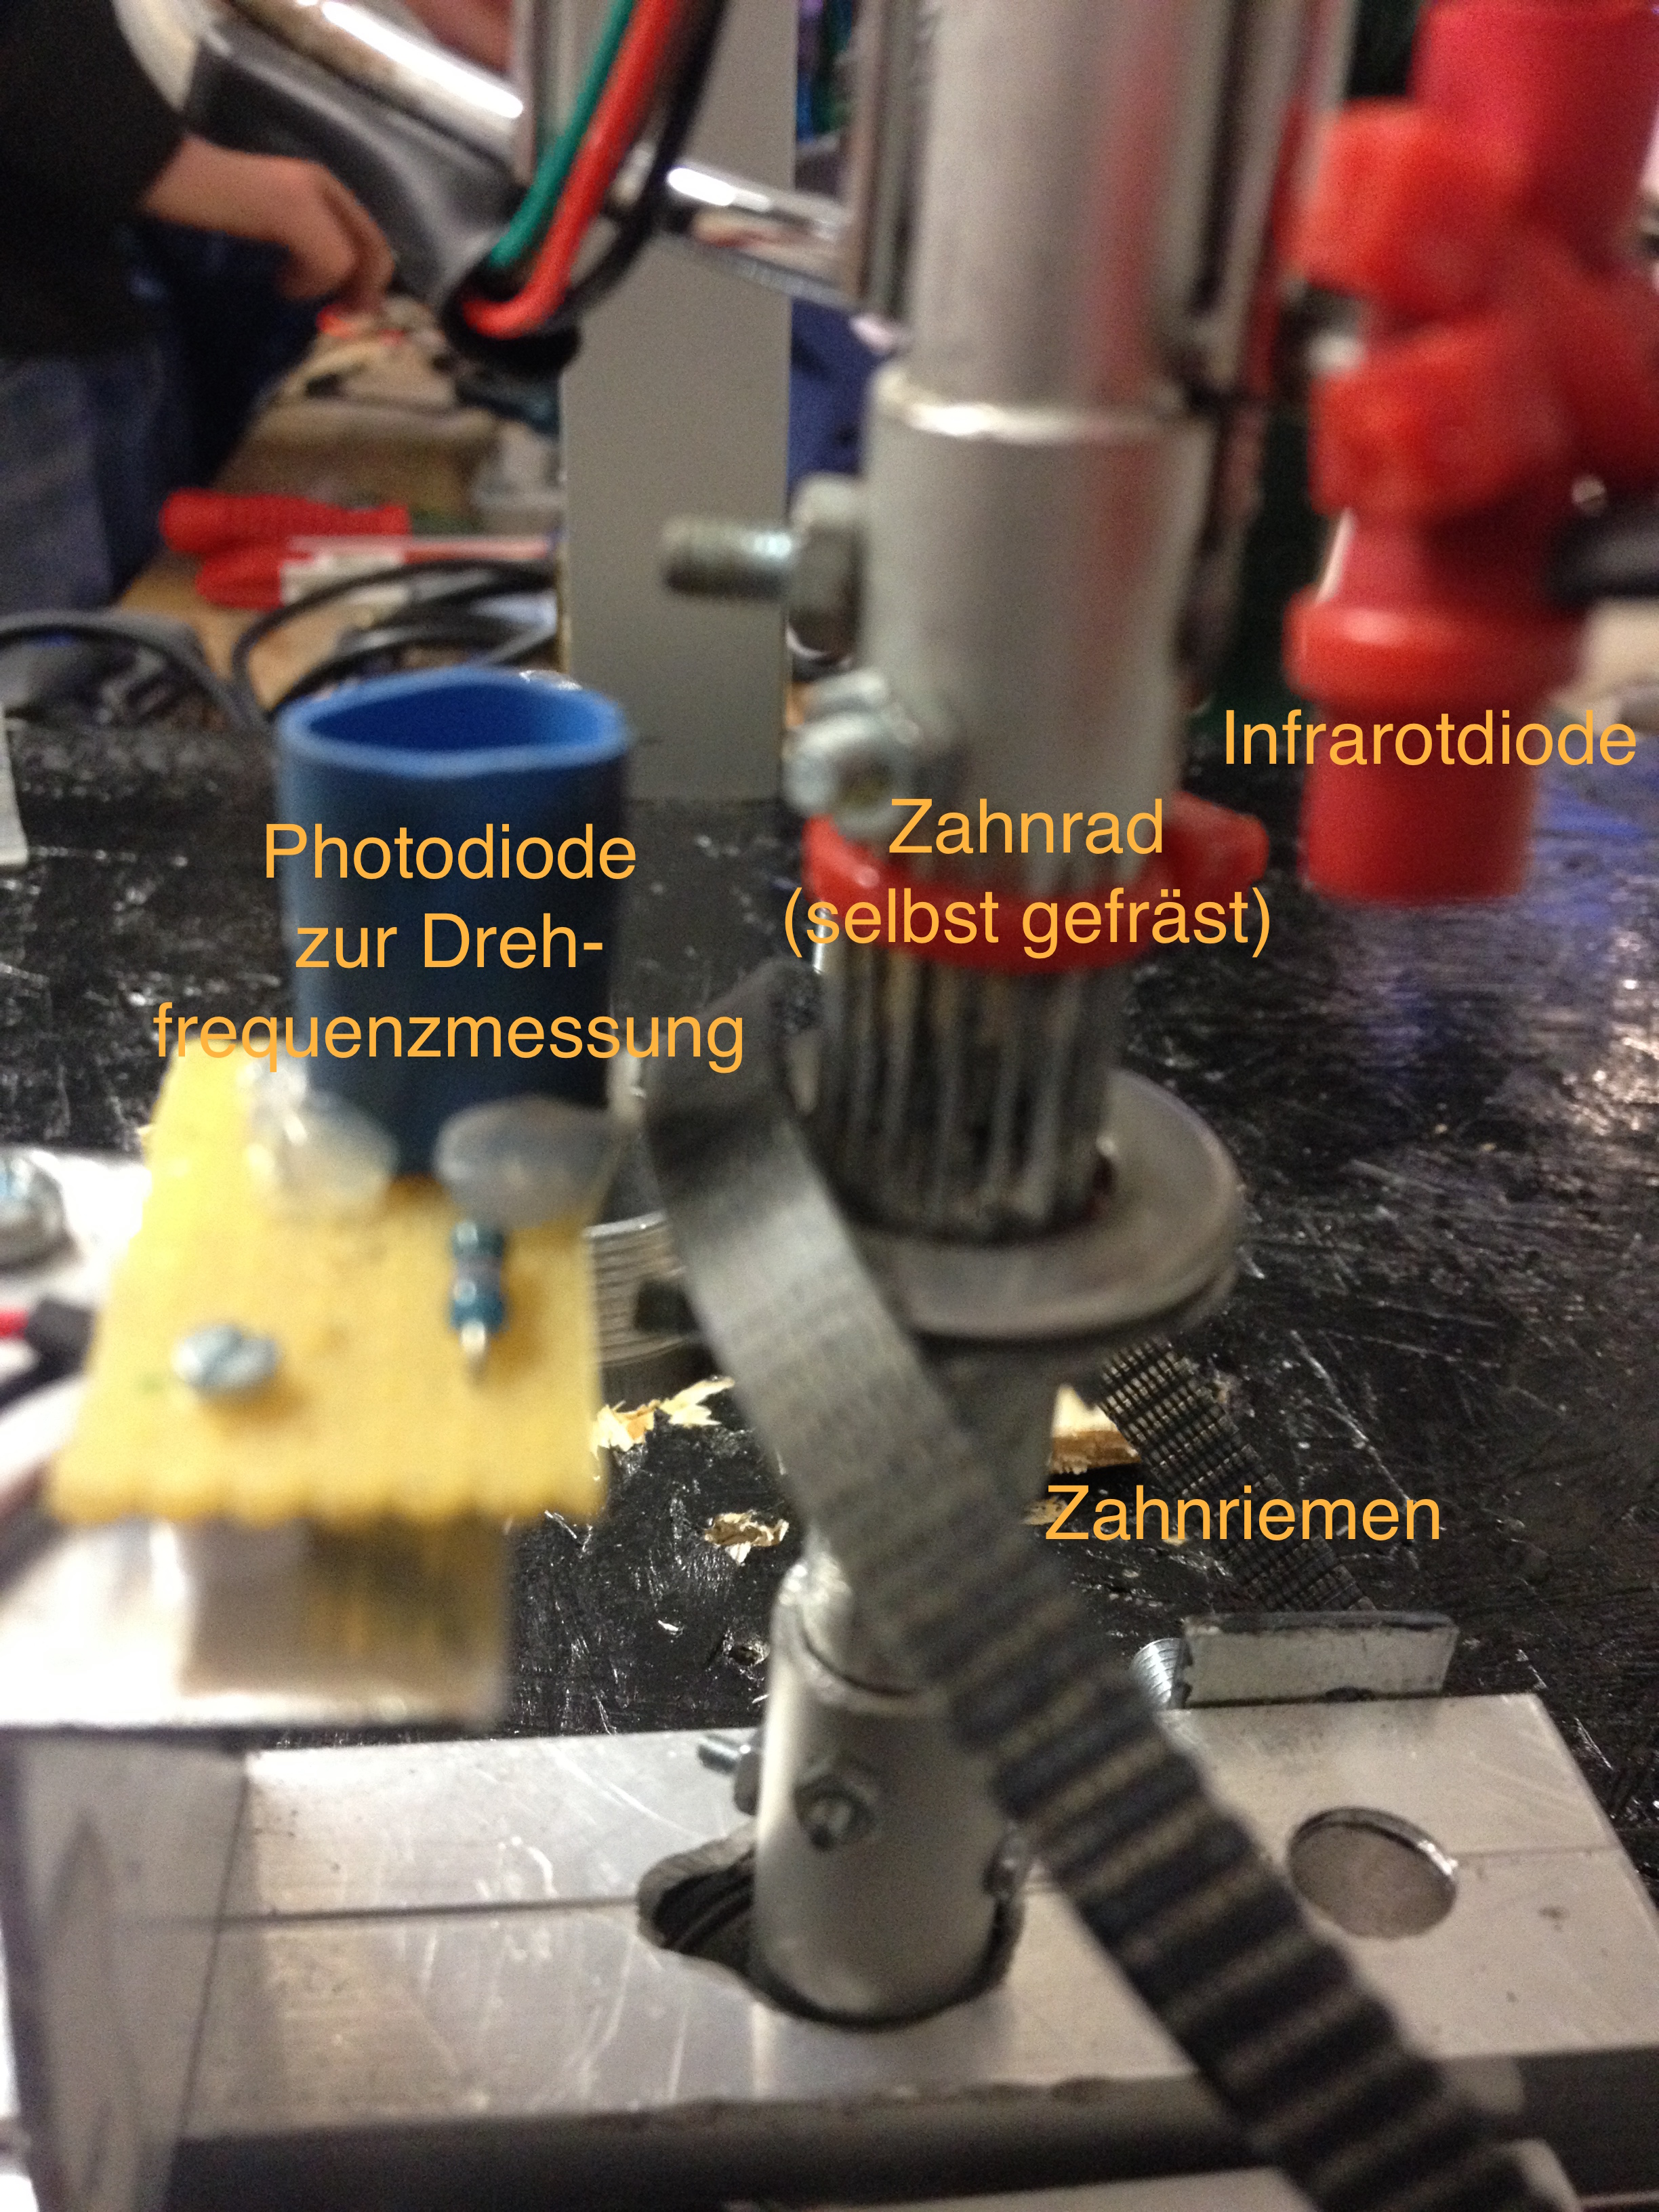
\includegraphics[height=9cm]{Bilder/Zahnriemen}
	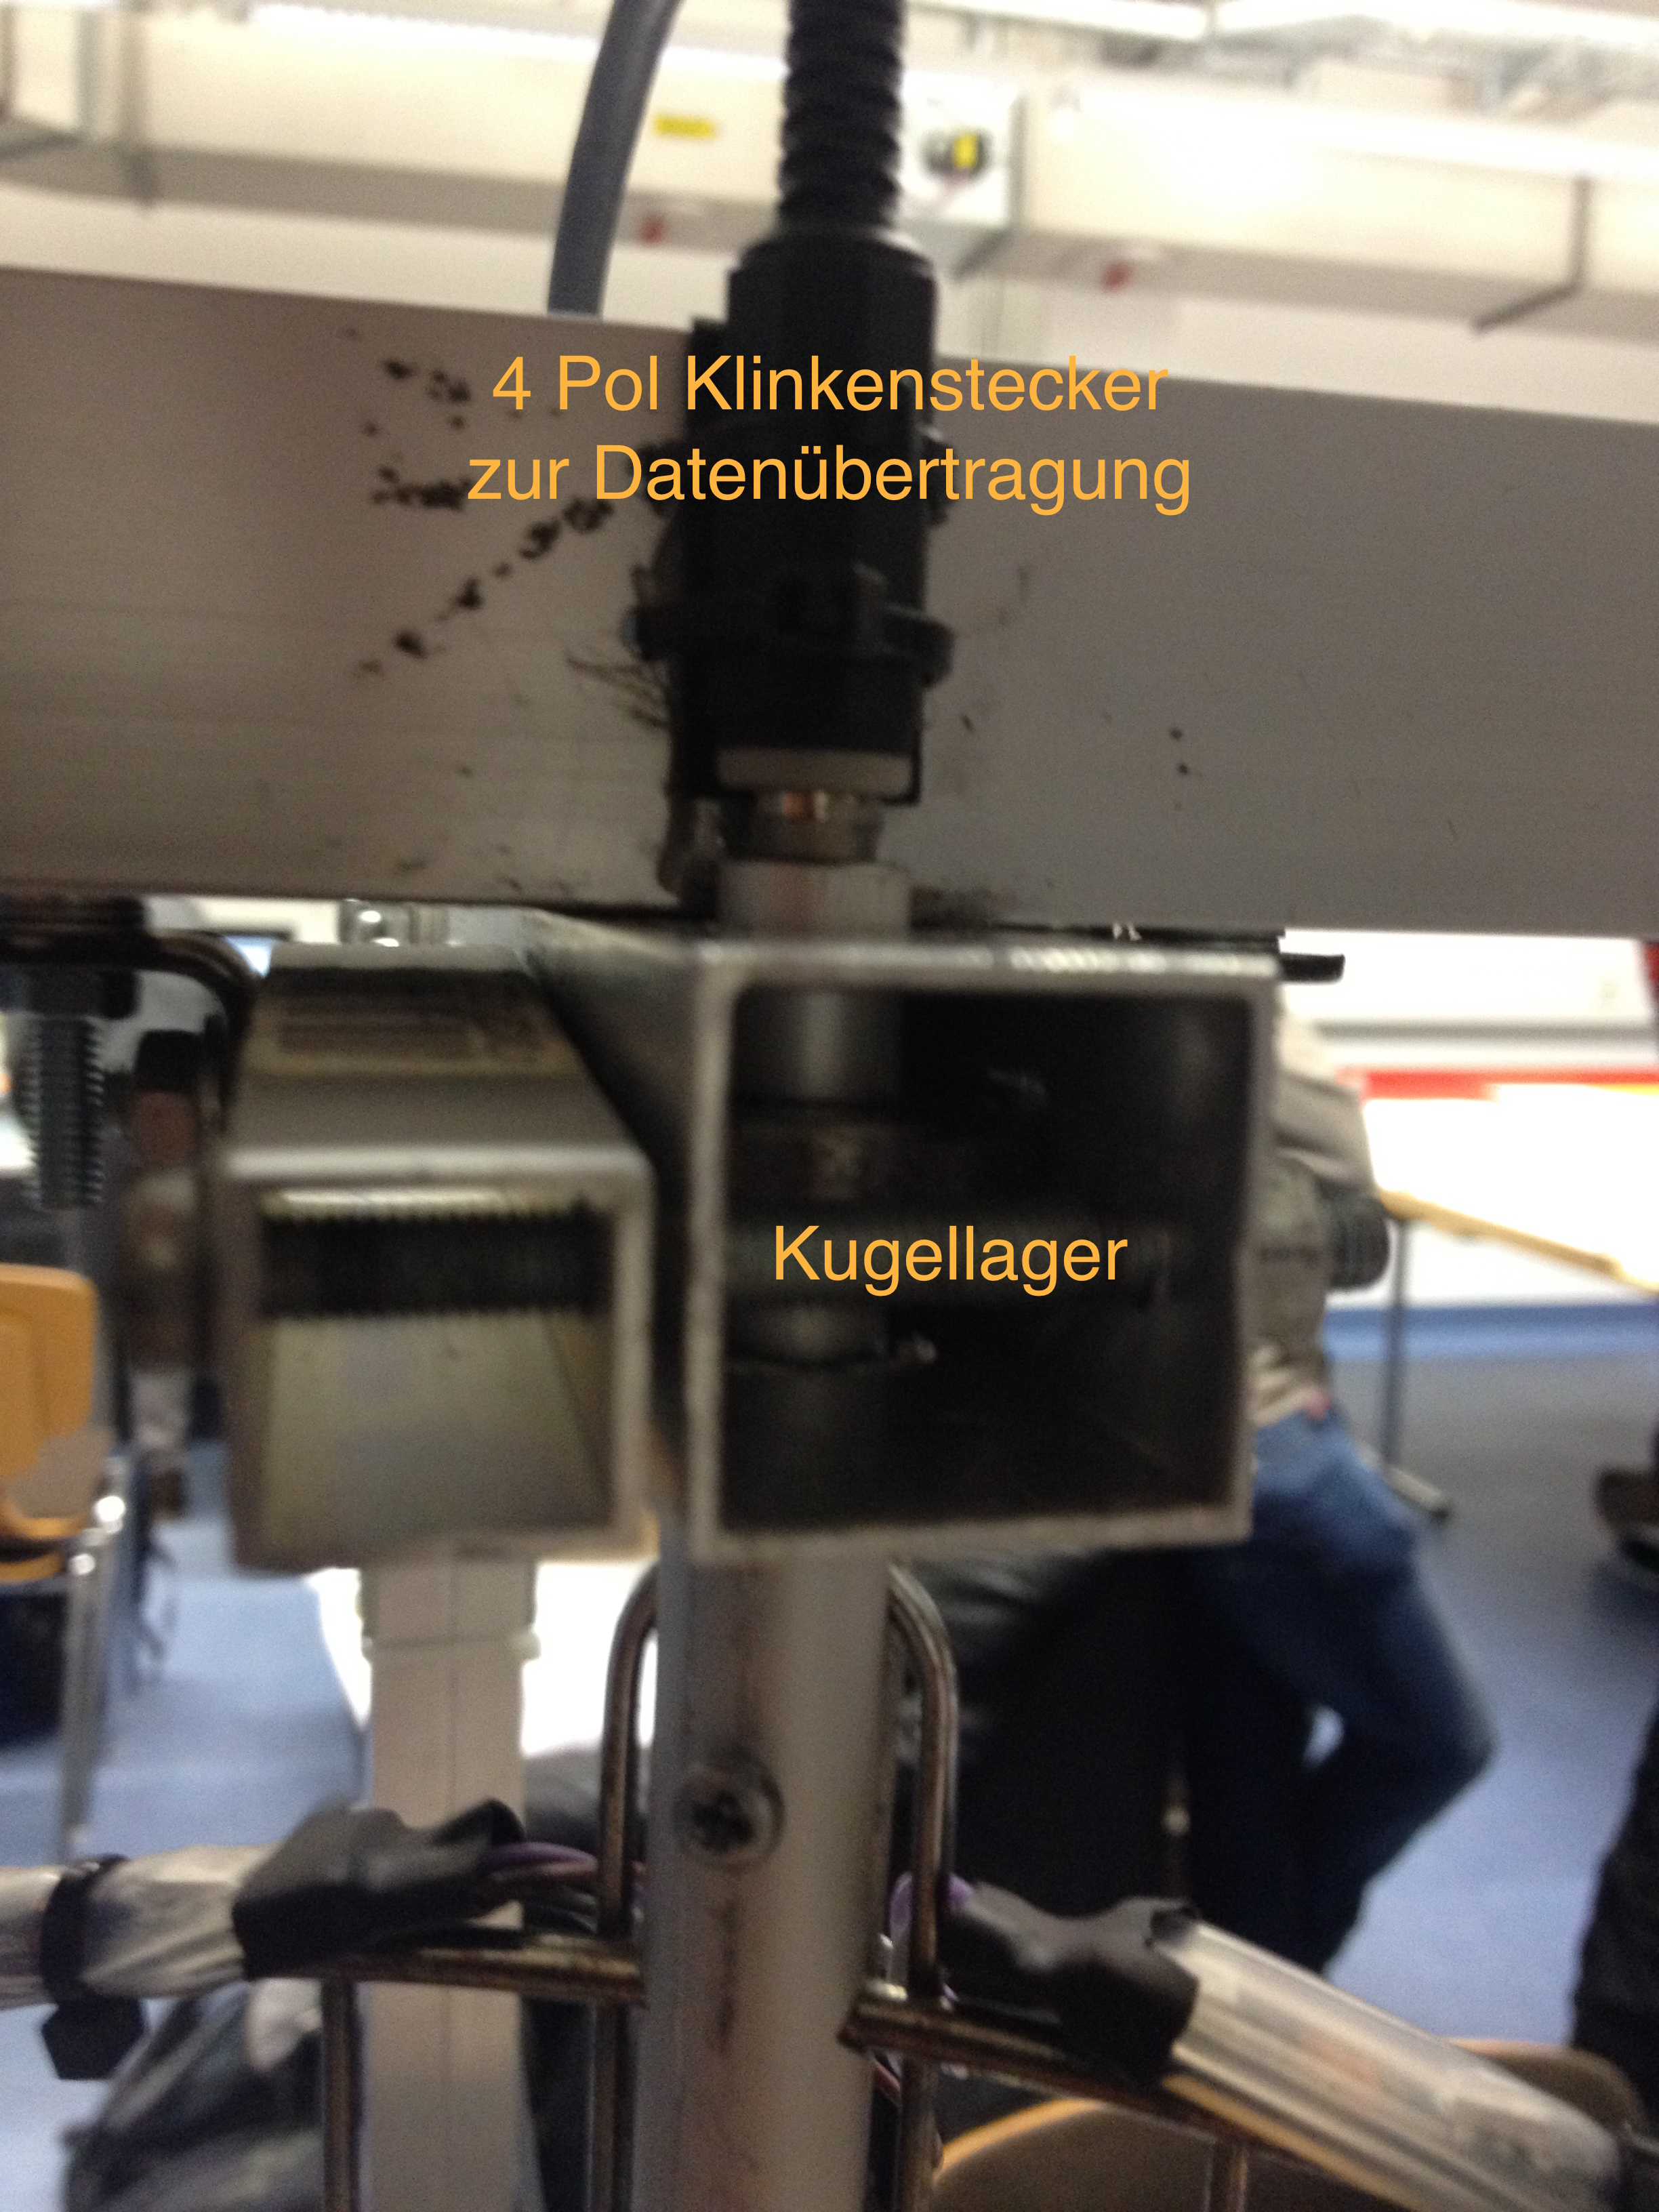
\includegraphics[height=9cm]{Bilder/Klinke}
\end{center}	
}

\headerbox{Weiterentwicklung}{name=ausblick,column=1,below=konzept}{
%Zur Weiterentwicklung bzw. Verbesserung des Roboters können folgende Punkte umgesetzt werden:
\begin{itemize}
\setlength\itemsep{-.3em}
%\vspace{-0.2cm}
	\item Verbesserung der Bildverarbeitung
	\vspace{-.55em}
	\begin{itemize}
	\setlength\itemsep{-.2em}
	\item bewegte Bilder
	\item Schrift / Laufschrift
	\end{itemize}
	\vspace{-.45em}
%\vspace{-0.65cm}
	\item Bessere Lagerung der drehenden Komponenten
%\vspace{-0.2cm}
	\item schneller/besserer Motor
%\vspace{-0.2cm}
	\item höhere Anzahl an Pixeln
\end{itemize}
%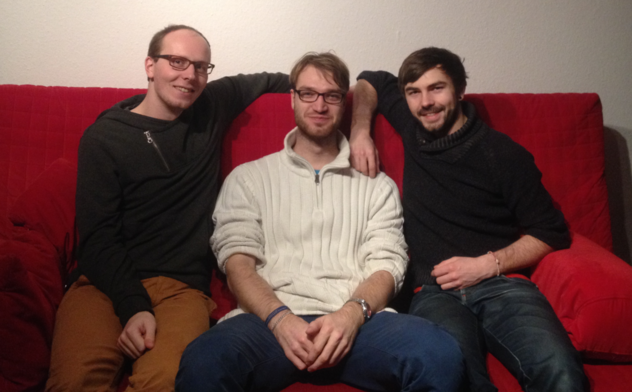
\includegraphics[angle=-90,width=0.49\linewidth]{team.jpg}
} 

\headerbox{Das Team}{name=team,column=2,below=konzept}{
%\smaller						% Make the whole text smaller
\vspace{0.1em}			% Save some space at the beginning
\begin{center}
Maximilian Hartmann\\
10. Semester Physik\\
%\vspace{0.3cm}
Philipp Gernandt\\
8. Semester Physik\\
Tobias Buck\\
10. Semester Physik\\
\vspace{0.1em}	
gps\_robotic@gmx.de
\vspace{0.1em}	
\end{center}
%\includegraphics[width=1\linewidth]{23uhr.jpg}
} 

\headerbox{Referenzen}{name=ref,span=2,column=1,above=bottom}{
\smaller						% Make the whole text smaller
\begin{multicols}{2}
https://github.com/TobiBu/POV\\
https://www.adafruit.com
\end{multicols}
} 

\end{poster}
\end{document}
